\documentclass[12pt,a4paper]{article}

\usepackage[utf8]{inputenc}
\usepackage[T1]{fontenc}
\usepackage[polish]{babel}
\usepackage{amsmath, amssymb, amsthm}
\usepackage{graphicx}
\usepackage{booktabs}
\usepackage{array}
\usepackage{geometry}
\usepackage{hyperref}
\usepackage{caption}
\usepackage{float}
\usepackage{xcolor}

\geometry{margin=2.5cm}
\graphicspath{{../src/problem_1/figures/}}

\hypersetup{
    colorlinks=true,
    linkcolor=black,
    urlcolor=blue,
    citecolor=black
}

\title{}
\author{}
\date{}

\begin{document}

\begin{titlepage}
    \centering
    \vspace*{2cm}

    {\Large Politechnika Warszawska}\\[0.3cm]
    {\large Wydział Elektroniki i Technik Informacyjnych}\\[2cm]

    {\large Statystyka w Analizie Danych}\\[0.5cm]
    {\large 01.06.2026}\\[1.5cm]

    \rule{\linewidth}{0.5mm}\\[0.4cm]
    {\huge\bfseries Projekt 2}\\[0.3cm]
    {\Large Testy zgodności rozkładu średniej z rozkładem normalnym\\
    oraz detekcja słabego sygnału w szumie}\\[0.2cm]
    \rule{\linewidth}{0.5mm}\\[2cm]

    \begin{flushright}
        \large
        \textit{Autorzy:}\\[0.4cm]
        Mikołaj Garbowski, nr albumu XXXXXX\\
        Bartłomiej Dmitruk, nr albumu 324911\\
    \end{flushright}

    \vfill
    {\large Warszawa, 2026}
\end{titlepage}

\tableofcontents
\newpage

\section{Problem 1 - CTG, kontynuacja Projektu 1}

\subsection{Metoda rozwiązania problemu}

Zadanie polega na ilościowym ujęciu zbieżności rozkładu średniej arytmetycznej $\bar{X}_n$ niezależnych zmiennych losowych do rozkładu normalnego, wynikającej z Centralnego Twierdzenia Granicznego. O ile w pierwszej części projektu zbieżność ta była pokazywana w sposób obrazowy (histogramy, estymatory jądrowe, dystrybuanty empiryczne, wykresy kwantyl-kwantyl), o tyle w tym problemie należy zbadać ją za pomocą statystycznych testów zgodności i porównać moce trzech klasycznych narzędzi: testu Kołmogorowa-Smirnowa, testu Shapiro-Wilka oraz testu D'Agostino. Wynikiem porównania ma być wskazanie, który test najskuteczniej wykrywa odchylenia rozkładu $\bar{X}_n$ od rozkładu normalnego w analizowanym przypadku. Uzupełnienie analizy stanowi estymacja skośności i kurtozy nadmiarowej $\bar{X}_n$ jako wielkości, na których wprost opiera się statystyka testu D'Agostino.

Wybór rozkładu bazowego padł na rozkład wykładniczy z parametrem $\lambda = 1$, czyli $X \sim \mathrm{Exp}(1)$. Decyzja ta wynika z dwóch przesłanek. Po pierwsze, rozkład wykładniczy jest silnie skośny (skośność równa $2$) i ma kurtozę nadmiarową $6$, dzięki czemu odchylenie $\bar{X}_n$ od rozkładu normalnego dla małych $n$ jest wyraźne, a jednocześnie zanika w znanym tempie. Po drugie, wszystkie istotne momenty są dane wzorami analitycznymi ($\mu = 1$, $\sigma^2 = 1$, $\mathrm{Skew}(\bar{X}_n) = 2/\sqrt{n}$, $\mathrm{ExcessKurt}(\bar{X}_n) = 6/n$), co pozwala bezpośrednio porównać estymaty empiryczne z teorią.

Strukturę eksperymentu opisują dwa różne parametry, których nie należy mylić. Liczba uśrednianych zmiennych $n$ wyznacza próbkę, której średnia ma być testowana - jej rosnące wartości odpowiadają coraz lepszemu dopasowaniu $\bar{X}_n$ do rozkładu normalnego. Liczba średnich $K$, podawana na wejście pojedynczego testu, opisuje, ile niezależnych realizacji $\bar{X}_n$ test otrzymuje naraz; im większe $K$, tym silniejszy test (lepsza zdolność wykrycia odchyleń). Zgodnie z zaleceniem projektowym przyjęto $K = 50$ - umiarkowaną wartość rzędu kilkudziesięciu. Liczba uśrednianych zmiennych przyjmuje wartości $n \in \{2, 3, 5, 7, 10, 15, 20, 30, 50, 70, 100, 200, 500\}$, co pokrywa całą strefę przejścia od małych prób, gdzie odchylenie od normalności jest wyraźne, aż do prób, dla których żaden z testów nie potrafi już rozróżnić $\bar{X}_n$ od $N(\mu, \sigma^2/n)$.

Schemat pojedynczej symulacji wygląda następująco. Dla ustalonego $n$ generowanych jest $K$ niezależnych prób o liczności $n$ z rozkładu $\mathrm{Exp}(1)$ i z każdej obliczana jest średnia arytmetyczna. Otrzymany wektor $K$ średnich stanowi wejście dla trzech testów normalności. Test Kołmogorowa-Smirnowa porównuje dystrybuantę empiryczną standaryzowanych średnich z dystrybuantą $N(0,1)$ przy znanych parametrach $\mu$ oraz $\sigma$, co zapewnia poprawny rozmiar testu i pozwala uniknąć poprawki Lillieforsa. Test Shapiro-Wilka opiera się na statystyce porównującej kombinację liniową statystyk pozycyjnych z wariancją próby i jest powszechnie uznawany za jeden z najmocniejszych testów normalności w niewielkich próbach. Test D'Agostino-Pearsona (statystyka $K^2$) łączy dwa składniki: jeden zależy od skośności, drugi od kurtozy, dzięki czemu test wprost wykrywa najczęstsze formy odejścia od normalności. Całość powtórzono $10\,000$ razy dla każdej wartości $n$, a frakcję odrzuceń hipotezy zerowej przy poziomie istotności $\alpha = 0{,}05$ przyjęto jako estymator mocy.

Aby zweryfikować poprawność implementacji oraz upewnić się, że wszystkie trzy testy utrzymują nominalny poziom istotności, równolegle przeprowadzono symulację kontrolną. W tej wersji $K$ średnich generowano bezpośrednio z rozkładu normalnego $N(0, 1)$ - hipoteza zerowa jest wtedy prawdziwa, a frakcja odrzuceń powinna być bliska $\alpha$. Odchylenia od $0{,}05$ większe niż wynikające z błędu Monte Carlo wskazywałyby na problem z implementacją lub niewłaściwą standaryzacją w teście Kołmogorowa-Smirnowa.

Estymację skośności i kurtozy nadmiarowej $\bar{X}_n$ przeprowadzono osobno, używając $100\,000$ niezależnych realizacji średniej dla każdej wartości $n$. Empiryczne wartości momentów porównano z formułami teoretycznymi $\mathrm{Skew}(\bar{X}_n) = 2/\sqrt{n}$ i $\mathrm{ExcessKurt}(\bar{X}_n) = 6/n$, właściwymi dla bazowego rozkładu $\mathrm{Exp}(1)$. Spadek skośności jak $1/\sqrt{n}$ oraz kurtozy jak $1/n$ odpowiada za stopniowy zanik mocy testu D'Agostino, którego statystyka właśnie z tych dwóch wielkości jest zbudowana.

Symulacje zaimplementowano w języku Python z wykorzystaniem bibliotek \texttt{numpy} oraz \texttt{scipy.stats}; testy wywołują funkcje \texttt{kstest}, \texttt{shapiro} i \texttt{normaltest}. Wszystkie generatory liczb pseudolosowych zainicjalizowano oddzielnymi ziarnami pochodnymi od stałej $\mathrm{SEED} = 42$, dzięki czemu wyniki są w pełni powtarzalne.

\subsection{Wyniki}

\subsubsection{Ilustracja zbieżności $\bar{X}_n$ do rozkładu normalnego}

Punktem wyjścia analizy jest wizualne potwierdzenie, że standaryzowana średnia $Z_n = (\bar{X}_n - \mu)/(\sigma/\sqrt{n})$ rzeczywiście zbiega do $N(0, 1)$ wraz ze wzrostem $n$. Rysunek~\ref{fig:convergence} przedstawia w górnym rzędzie histogramy gęstości $Z_n$ uzyskane ze $100\,000$ niezależnych realizacji dla czterech wybranych wartości $n \in \{2, 10, 50, 200\}$, a w dolnym - odpowiadające im wykresy kwantyl-kwantyl względem rozkładu $N(0, 1)$. Dla $n = 2$ histogram zachowuje wyraźną prawostronną skośność dziedziczoną z rozkładu wykładniczego: wartość modalna leży po lewej stronie zera, prawy ogon jest znacznie wydłużony, a wykres kwantyl-kwantyl odchyla się od prostej w obu krańcach, najmocniej w prawym ogonie. Dla $n = 10$ asymetria histogramu wyraźnie się zmniejsza, a wykres kwantyl-kwantyl niemal pokrywa się z prostą w centralnej części, odchylenia pozostają jednak widoczne w prawym ogonie. Przy $n = 50$ histogram jest praktycznie symetryczny i bardzo dobrze odpowiada krzywej gęstości $N(0, 1)$, a wykres kwantyl-kwantyl tworzy linię praktycznie nieodróżnialną od idealnej diagonali. Dla $n = 200$ dopasowanie jest tak dobre, że żadnym z dwóch sposobów nie sposób gołym okiem stwierdzić odejścia od normalności - i właśnie tu pojawia się potrzeba zastosowania testów statystycznych, które jako jedyne dają obiektywną, ilościową odpowiedź na pytanie, czy odchylenie jest jeszcze wykrywalne.

\begin{figure}[H]
    \centering
    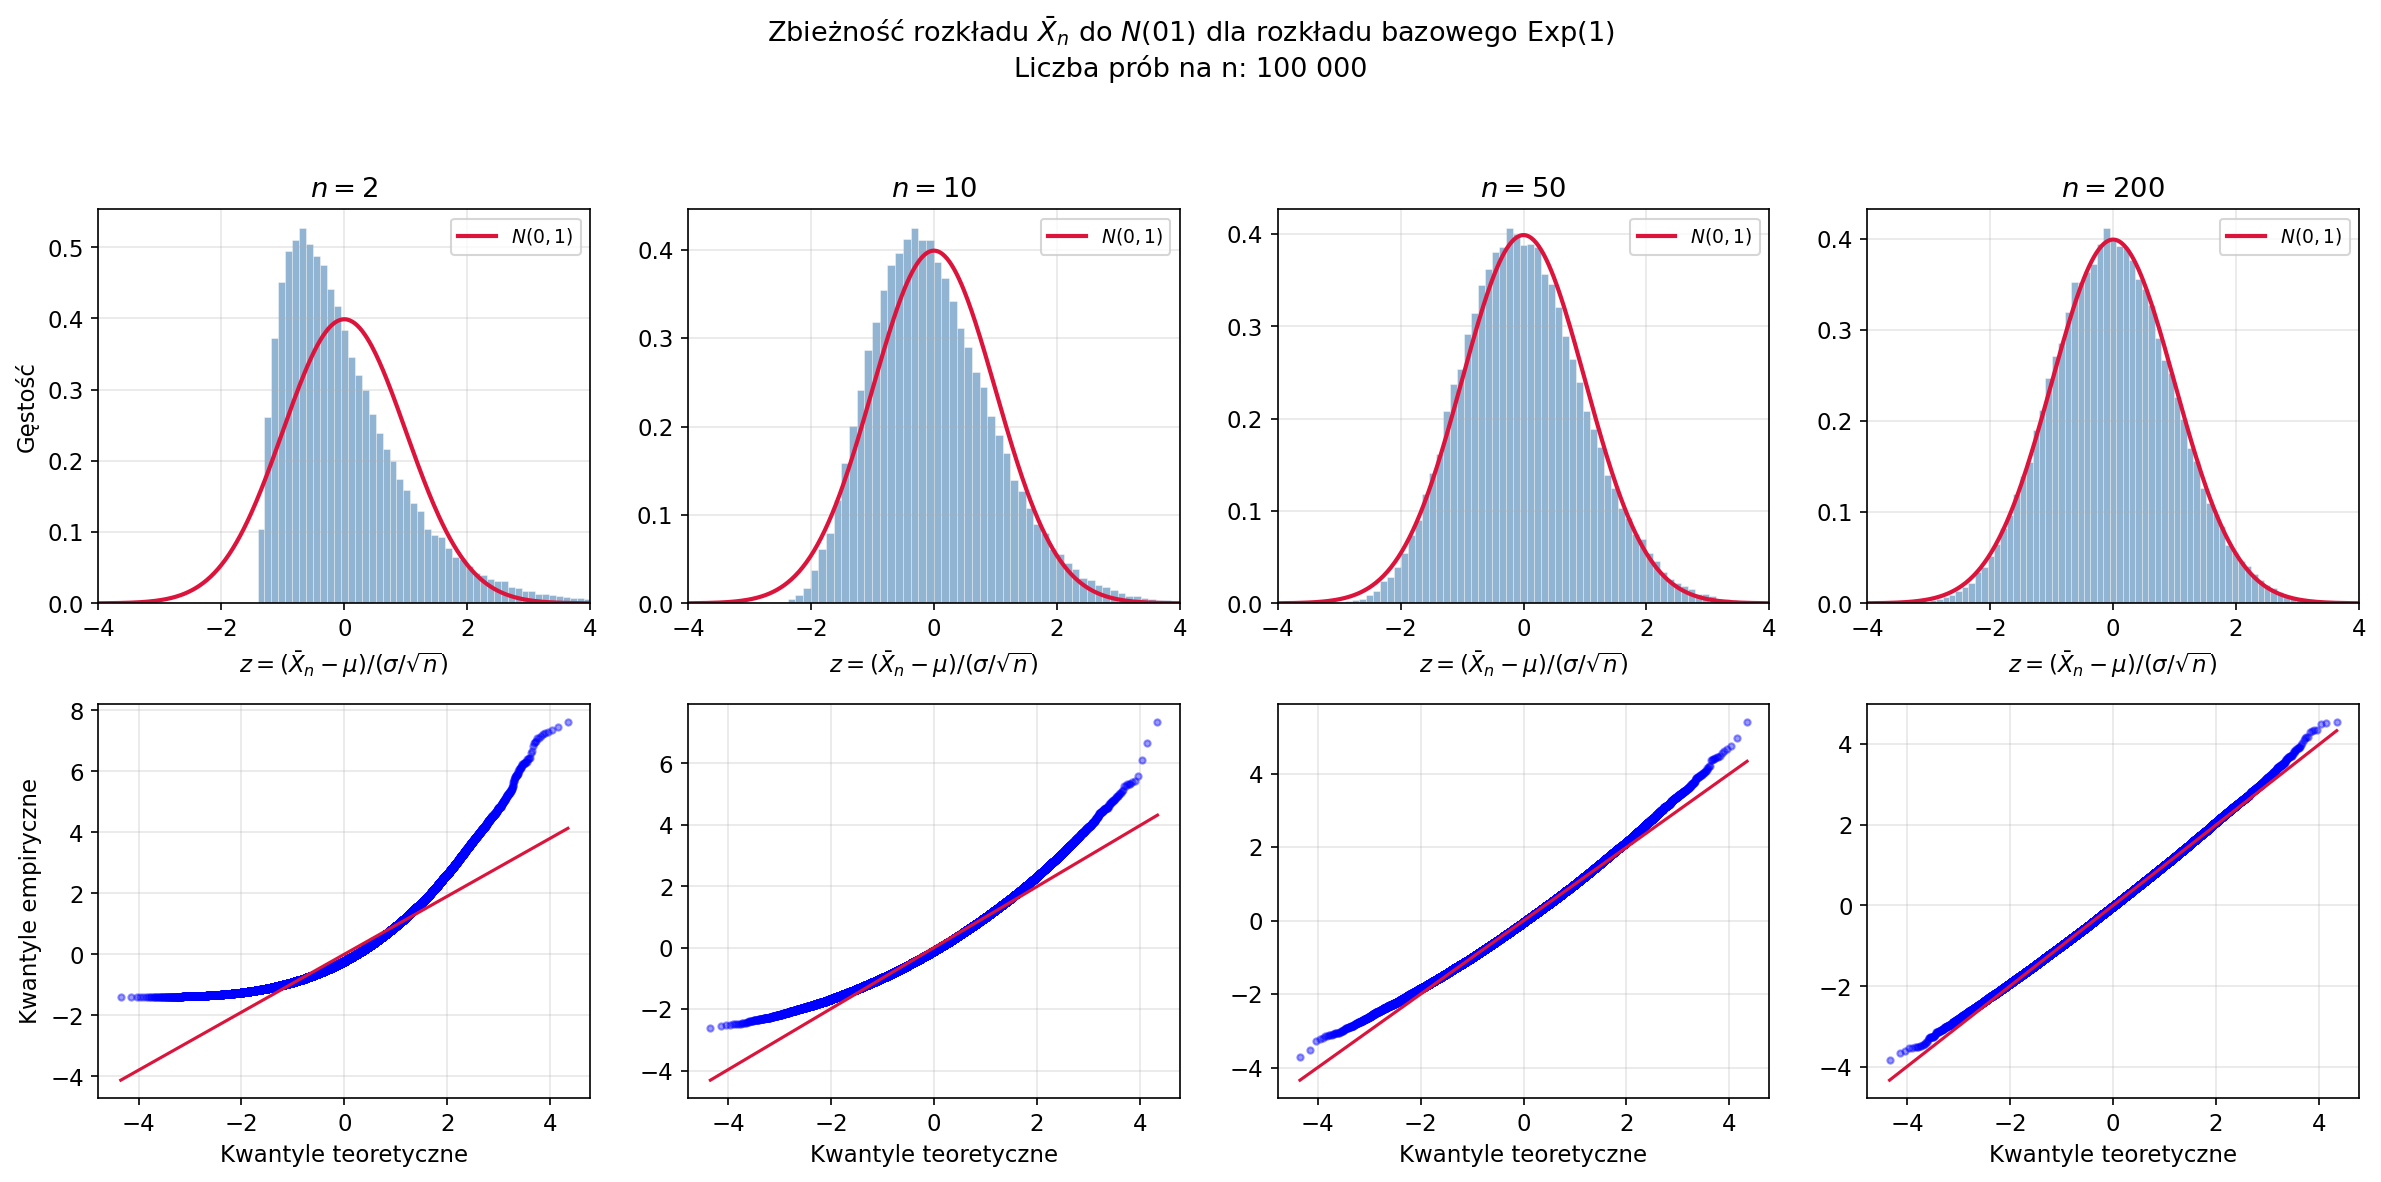
\includegraphics[width=\textwidth]{convergence.png}
    \caption{Zbieżność standaryzowanej średniej $Z_n = (\bar{X}_n - \mu)/(\sigma/\sqrt{n})$ z rozkładu bazowego $\mathrm{Exp}(1)$ do rozkładu $N(0, 1)$. Górny rząd: histogramy gęstości na tle teoretycznej krzywej $N(0, 1)$. Dolny rząd: wykresy kwantyl-kwantyl względem rozkładu $N(0, 1)$.}
    \label{fig:convergence}
\end{figure}

\subsubsection{Moc testów normalności}

Centralny wynik pracy stanowi porównanie mocy trzech testów. Rysunek~\ref{fig:power} pokazuje empiryczną frakcję odrzuceń hipotezy zerowej w funkcji liczby uśrednianych zmiennych $n$, przy stałym $K = 50$ i $\alpha = 0{,}05$. Wszystkie trzy krzywe są monotonicznie malejące - wraz ze wzrostem $n$ rozkład $\bar{X}_n$ coraz lepiej naśladuje rozkład normalny, więc testom jest coraz trudniej wykryć odchylenie od $N(\mu, \sigma^2/n)$.

\begin{figure}[H]
    \centering
    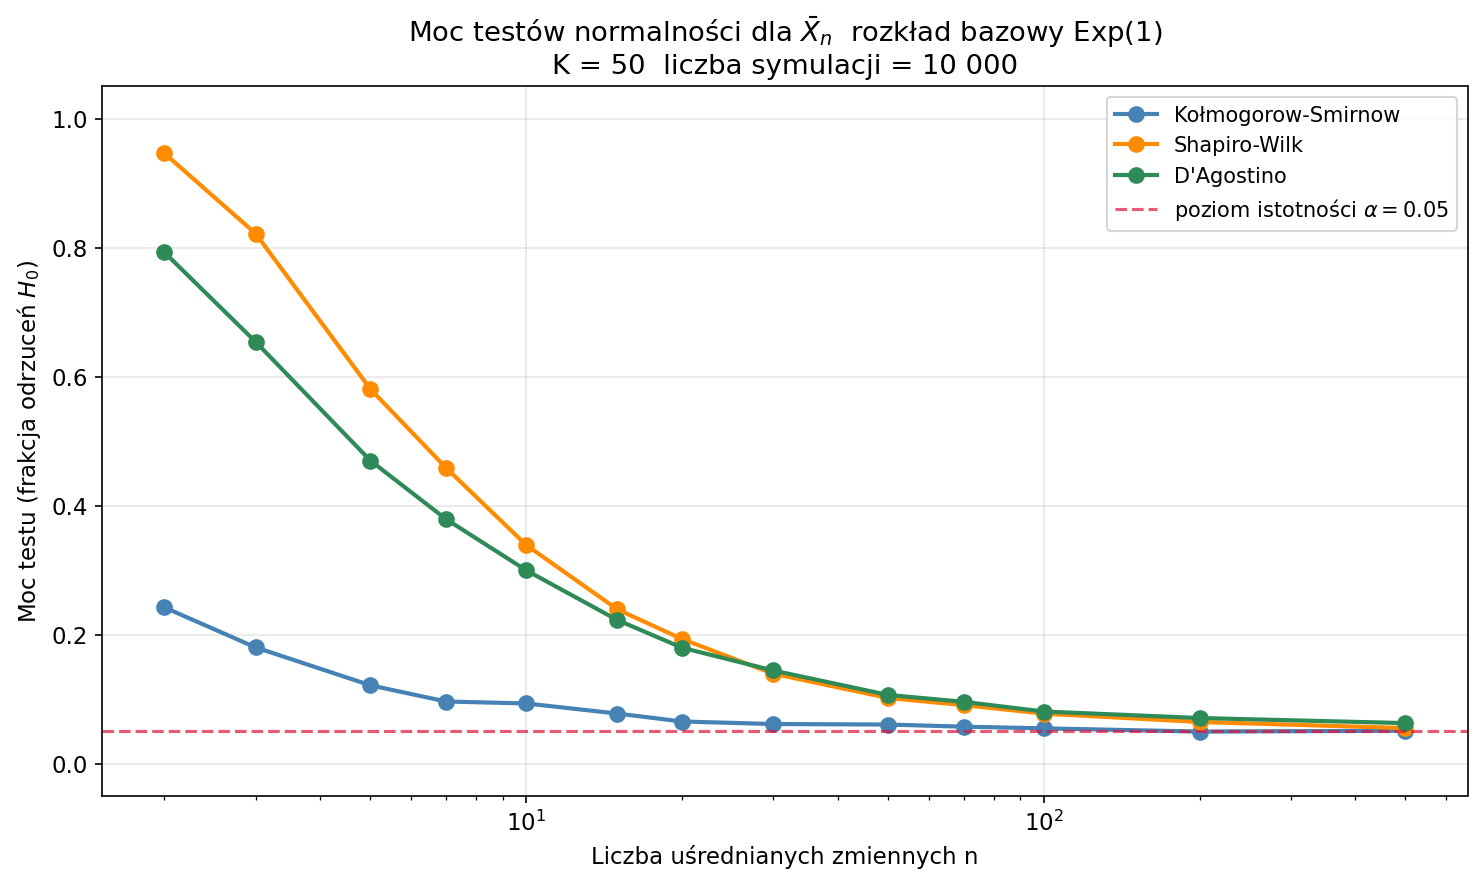
\includegraphics[width=\textwidth]{power_curves.png}
    \caption{Moc testów normalności (frakcja odrzuceń $H_0$) dla średniej $\bar{X}_n$ z rozkładu $\mathrm{Exp}(1)$, $K = 50$, $\alpha = 0{,}05$, $10\,000$ symulacji.}
    \label{fig:power}
\end{figure}

Już z tego rysunku widać wyraźną hierarchię testów. Test Shapiro-Wilka odrzuca hipotezę zerową przy $n = 2$ w niemal 95\% przypadków, podczas gdy test D'Agostino osiąga w tej samej sytuacji moc na poziomie 79\%, a test Kołmogorowa-Smirnowa jedynie nieco ponad 24\%. Hierarchia ta utrzymuje się we wszystkich badanych wartościach $n$, choć przewaga testu Shapiro-Wilka nad D'Agostino jest stała i niewielka, natomiast przewaga obu nad testem Kołmogorowa-Smirnowa jest wielokrotna. Dla $n = 50$, czyli przypadku $K = n$, moce testów Shapiro-Wilka i D'Agostino spadają do około 10\%, a test Kołmogorowa-Smirnowa rejestruje już wartości w okolicach poziomu istotności - dla próby tej długości żaden z testów praktycznie nie odróżnia $\bar{X}_n$ od rozkładu normalnego.

Bliższy widok strefy przejściowej daje rysunek~\ref{fig:power_zoom}, na którym dodano linię referencyjną na poziomie mocy 0{,}5. Pozwala on odczytać, dla jakiej wartości $n$ dany test zachowuje co najmniej połowiczną zdolność wykrycia odchylenia. Test Shapiro-Wilka utrzymuje moc powyżej 0{,}5 do około $n \approx 7$, test D'Agostino nieznacznie krócej - do mniej więcej $n \approx 5$, natomiast moc testu Kołmogorowa-Smirnowa nigdy w badanym zakresie tej granicy nie przekracza i już przy $n = 2$ pozostaje na poziomie ok. 0{,}24.

\begin{figure}[H]
    \centering
    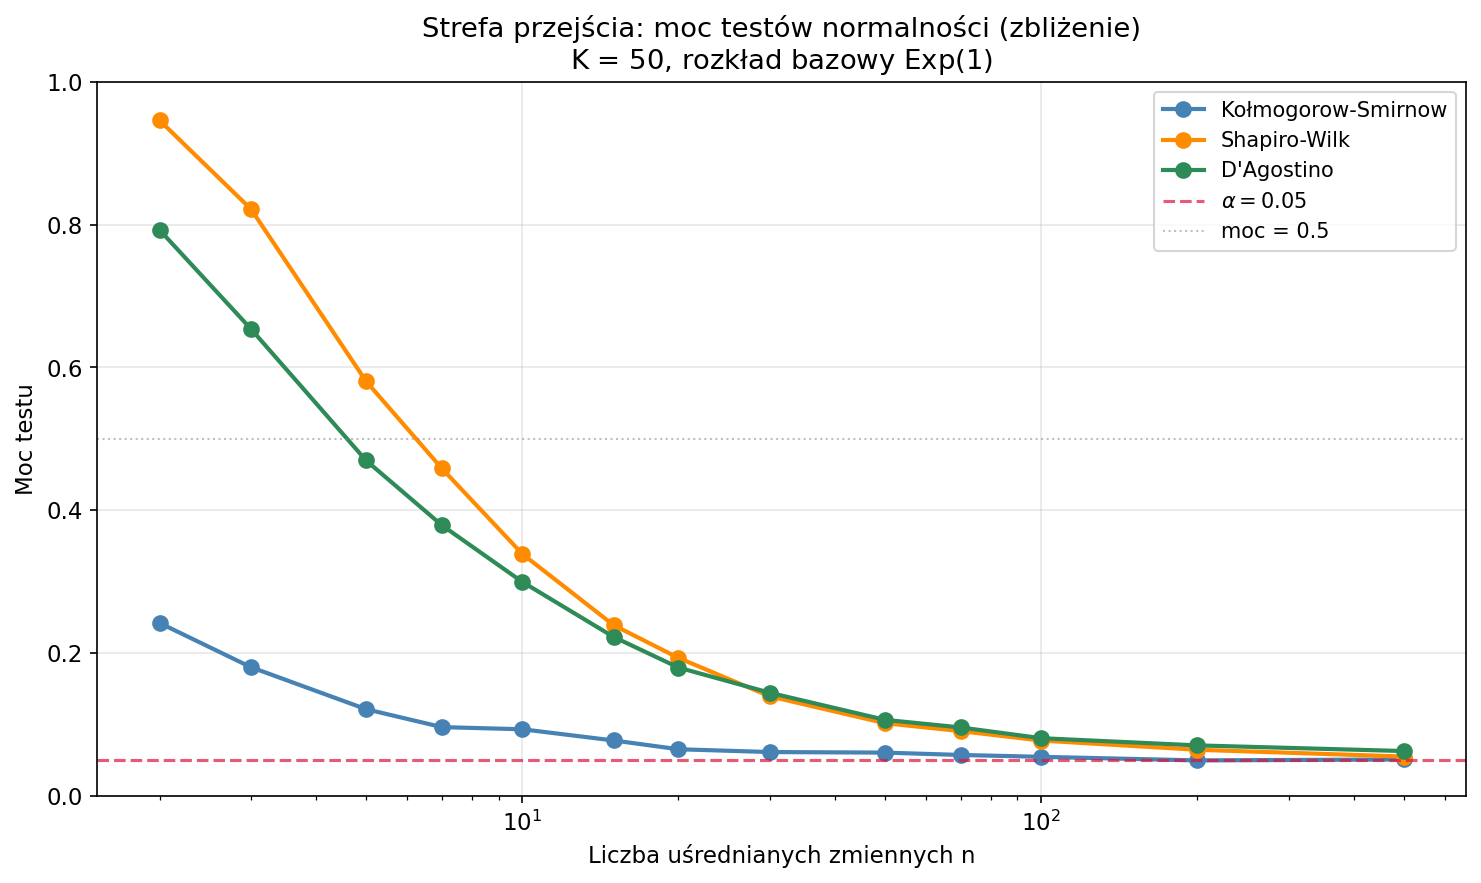
\includegraphics[width=\textwidth]{power_zoom.png}
    \caption{Strefa przejścia mocy testów normalności w pełnym zakresie pionowym z linią referencyjną na poziomie mocy 0{,}5, ułatwiającą porównanie tempa zaniku mocy między testami.}
    \label{fig:power_zoom}
\end{figure}

Pełne wartości liczbowe mocy testów zebrano w tabeli~\ref{tab:power}. W tej samej tabeli umieszczono również wyniki kontroli błędu I rodzaju - frakcję odrzuceń przy danych pochodzących z rozkładu $N(0, 1)$, kiedy hipoteza zerowa jest prawdziwa. Wartości te powinny być bliskie nominalnemu poziomowi istotności $\alpha = 0{,}05$, co rzeczywiście potwierdzają wyniki. Testy Kołmogorowa-Smirnowa i Shapiro-Wilka utrzymują empiryczny rozmiar praktycznie identyczny z nominalnym (różnice mieszczą się w zakresie szumu Monte Carlo), test D'Agostino nieznacznie odrzuca częściej (wartości w przedziale ok. $0{,}055$-$0{,}061$). Pełna zgodność z $\alpha$ stanowi potwierdzenie, że standaryzacja w teście Kołmogorowa-Smirnowa oraz cała procedura symulacyjna są zaimplementowane poprawnie, a różnice w mocach widoczne na rysunku~\ref{fig:power} wynikają faktycznie z odmiennej charakterystyki samych testów, nie z błędu metodologicznego.

\begin{table}[H]
    \centering
    \caption{Moc testów normalności dla danych $\bar{X}_n$ z $\mathrm{Exp}(1)$ oraz empiryczny rozmiar testów dla danych z $N(0, 1)$. $K = 50$, $\alpha = 0{,}05$, $10\,000$ symulacji.}
    \label{tab:power}
    \begin{tabular}{r|rrr|rrr}
\toprule
 & \multicolumn{3}{c|}{Moc (dane z Exp(1))} & \multicolumn{3}{c}{Empiryczny $\alpha$ (dane z $N(0,1)$)} \\
$n$ & KS & SW & D'A & KS & SW & D'A \\
\midrule
2 & 0.242 & 0.946 & 0.792 & 0.048 & 0.053 & 0.059 \\
3 & 0.180 & 0.822 & 0.654 & 0.049 & 0.050 & 0.055 \\
5 & 0.121 & 0.581 & 0.470 & 0.049 & 0.046 & 0.058 \\
7 & 0.096 & 0.459 & 0.379 & 0.050 & 0.054 & 0.058 \\
10 & 0.093 & 0.339 & 0.300 & 0.051 & 0.050 & 0.055 \\
15 & 0.078 & 0.239 & 0.223 & 0.053 & 0.050 & 0.055 \\
20 & 0.065 & 0.193 & 0.180 & 0.052 & 0.049 & 0.057 \\
30 & 0.061 & 0.139 & 0.144 & 0.053 & 0.049 & 0.054 \\
50 & 0.061 & 0.102 & 0.106 & 0.052 & 0.052 & 0.056 \\
70 & 0.057 & 0.091 & 0.096 & 0.049 & 0.051 & 0.059 \\
100 & 0.055 & 0.077 & 0.081 & 0.049 & 0.049 & 0.057 \\
200 & 0.050 & 0.065 & 0.071 & 0.048 & 0.050 & 0.061 \\
500 & 0.051 & 0.055 & 0.063 & 0.052 & 0.051 & 0.057 \\
\bottomrule
\end{tabular}

\end{table}

Rysunek~\ref{fig:type1} przedstawia te same liczby w postaci wykresu. Empiryczne rozmiary testów stabilnie oscylują wokół poziomu $0{,}05$ niezależnie od $n$, co świadczy o tym, że żaden z testów nie traci poprawności dla próbek o liczności $K = 50$.

\begin{figure}[H]
    \centering
    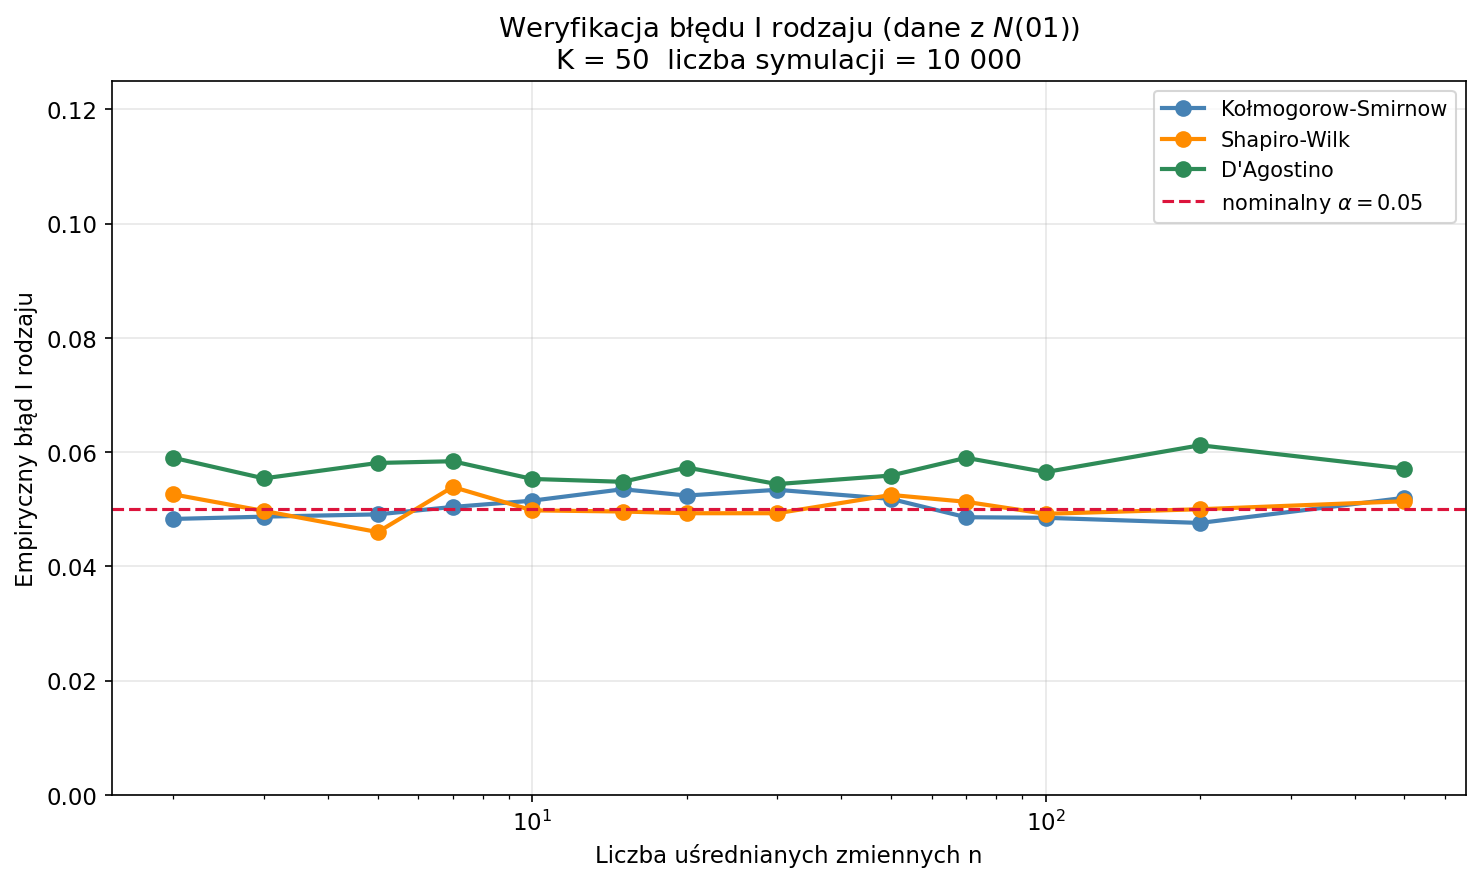
\includegraphics[width=\textwidth]{type_one_error.png}
    \caption{Weryfikacja błędu I rodzaju: empiryczna frakcja odrzuceń $H_0$ dla danych pochodzących z $N(0, 1)$ w funkcji $n$. Wszystkie krzywe oscylują w pobliżu nominalnego $\alpha = 0{,}05$.}
    \label{fig:type1}
\end{figure}

\subsubsection{Estymacja skośności i kurtozy nadmiarowej $\bar{X}_n$}

Dla pełnego zrozumienia, dlaczego test D'Agostino przestaje wykrywać odchylenia od normalności wraz ze wzrostem $n$, kluczowe są dwie wielkości, na których opiera się jego statystyka: skośność $g_1$ oraz kurtoza nadmiarowa $g_2$. Rysunek~\ref{fig:moments} przedstawia ich estymaty empiryczne wraz z krzywymi teoretycznymi $2/\sqrt{n}$ i $6/n$ właściwymi dla średniej z rozkładu $\mathrm{Exp}(1)$.

\begin{figure}[H]
    \centering
    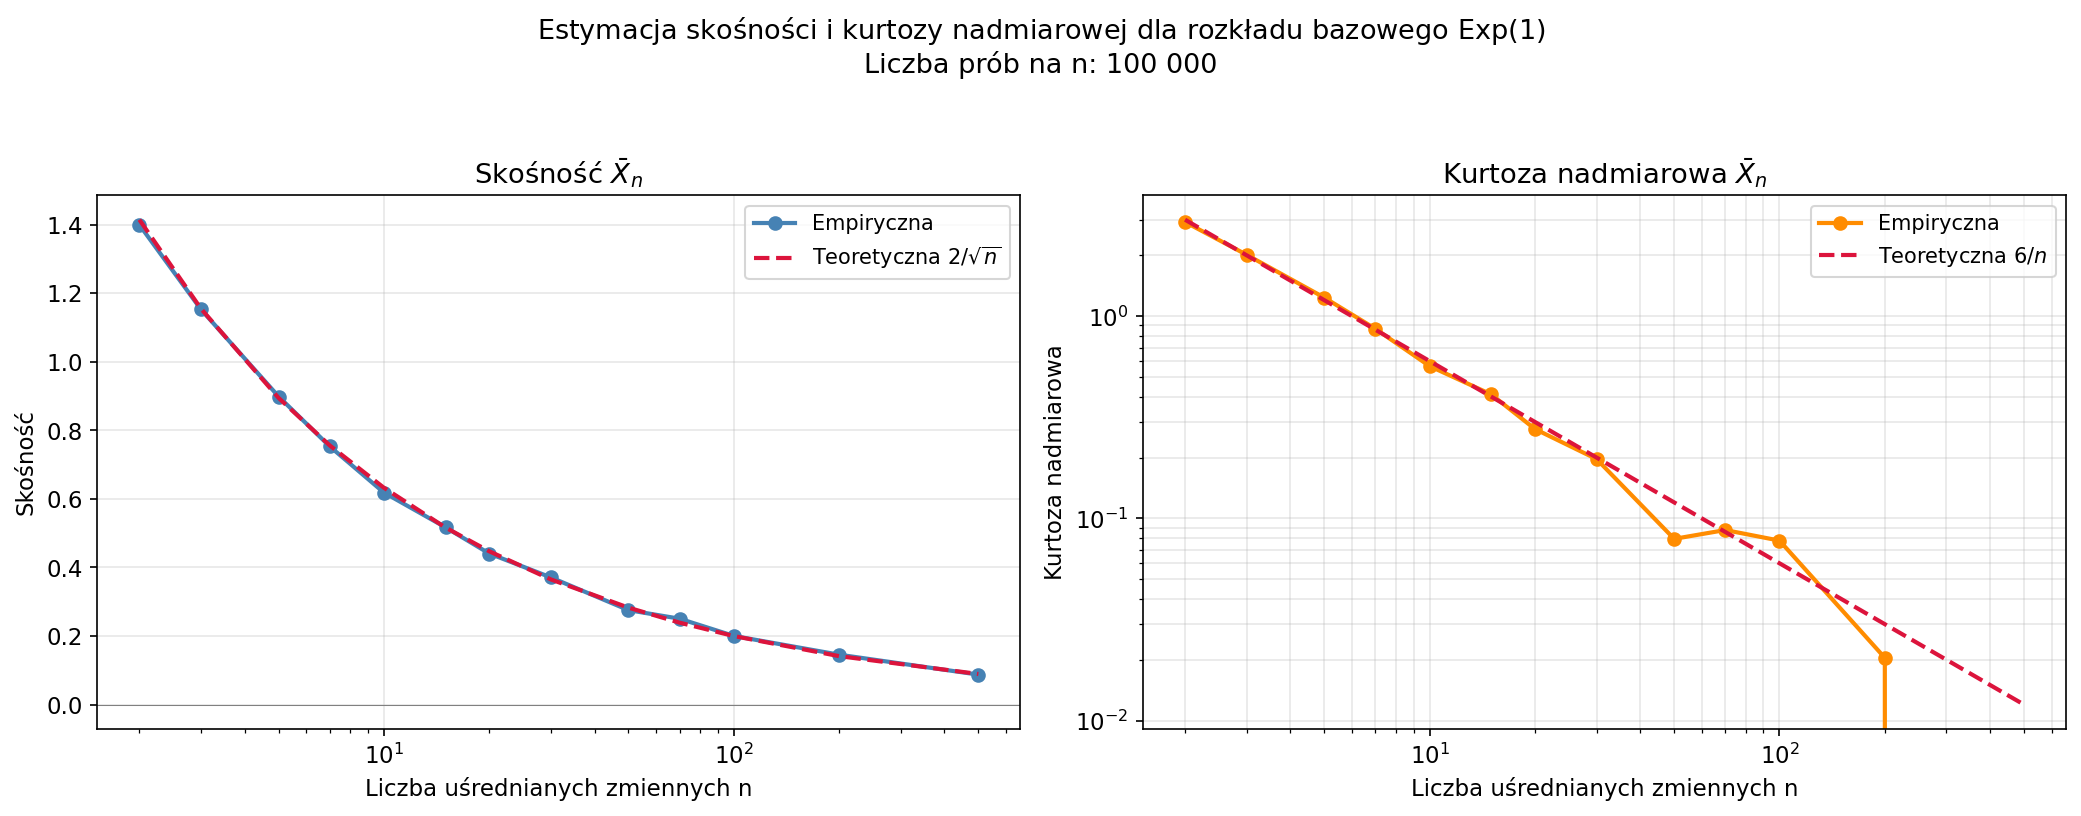
\includegraphics[width=\textwidth]{moments.png}
    \caption{Estymacja skośności (panel lewy) i kurtozy nadmiarowej (panel prawy) średniej $\bar{X}_n$ z rozkładu $\mathrm{Exp}(1)$. Punkty - wartości empiryczne (po $100\,000$ realizacji $\bar{X}_n$ dla każdego $n$); linie przerywane - teoretyczne $2/\sqrt{n}$ oraz $6/n$.}
    \label{fig:moments}
\end{figure}

Lewy panel pokazuje skośność. Punkty empiryczne pokrywają się z krzywą $2/\sqrt{n}$ z dokładnością odpowiadającą szumowi Monte Carlo - dla $n = 2$ wartość empiryczna wynosi $1{,}40$ przy teoretycznej $1{,}41$, dla $n = 30$ jest to $0{,}37$ wobec $0{,}37$, a dla $n = 500$ empiryczna skośność spada do $0{,}09$, w pełnej zgodzie z teorią. Prawy panel, w skali logarytmicznej na obu osiach, ilustruje analogiczne zachowanie kurtozy nadmiarowej: empiryczne wartości układają się wzdłuż linii prostej o nachyleniu odpowiadającym $1/n$. Dla największych $n$ punkty zaczynają nieznacznie odbiegać od linii teoretycznej - jest to efekt rosnącego względnego błędu estymatora kurtozy, gdy szacowana wartość zbliża się do zera (przy $n = 500$ teoretyczna kurtoza nadmiarowa wynosi $0{,}012$, więc nawet niewielka odchyłka empiryczna staje się widoczna w skali logarytmicznej).

Pełne wartości liczbowe zebrano w tabeli~\ref{tab:moments}.

\begin{table}[H]
    \centering
    \caption{Skośność i kurtoza nadmiarowa średniej $\bar{X}_n$ z rozkładu $\mathrm{Exp}(1)$: empiryczne wartości z $100\,000$ realizacji dla każdego $n$ i krzywe teoretyczne.}
    \label{tab:moments}
    \begin{tabular}{r|rr|rr}
\toprule
 & \multicolumn{2}{c|}{Skośność} & \multicolumn{2}{c}{Kurtoza nadmiarowa} \\
$n$ & empiryczna & teoretyczna $2/\sqrt{n}$ & empiryczna & teoretyczna $6/n$ \\
\midrule
2 & 1.3993 & 1.4142 & 2.9220 & 3.0000 \\
3 & 1.1525 & 1.1547 & 2.0117 & 2.0000 \\
5 & 0.8986 & 0.8944 & 1.2356 & 1.2000 \\
7 & 0.7531 & 0.7559 & 0.8661 & 0.8571 \\
10 & 0.6184 & 0.6325 & 0.5663 & 0.6000 \\
15 & 0.5170 & 0.5164 & 0.4103 & 0.4000 \\
20 & 0.4407 & 0.4472 & 0.2767 & 0.3000 \\
30 & 0.3710 & 0.3651 & 0.1966 & 0.2000 \\
50 & 0.2755 & 0.2828 & 0.0792 & 0.1200 \\
70 & 0.2506 & 0.2390 & 0.0876 & 0.0857 \\
100 & 0.2004 & 0.2000 & 0.0777 & 0.0600 \\
200 & 0.1456 & 0.1414 & 0.0204 & 0.0300 \\
500 & 0.0875 & 0.0894 & -0.0016 & 0.0120 \\
\bottomrule
\end{tabular}

\end{table}

\subsection{Interpretacja wyników i wnioski}

Wyniki symulacji prowadzą do kilku spójnych obserwacji, które łącznie odpowiadają na pytanie postawione w treści zadania.

Najwyższą moc w analizowanym przypadku wykazuje test Shapiro-Wilka. Jego przewaga jest widoczna w całym zakresie $n$ i wynika z konstrukcji statystyki: porównanie kombinacji liniowej statystyk pozycyjnych z wariancją próby jest czułe zarówno na asymetrię, jak i na ciężkie ogony rozkładu, a niewielkie $K$ (rzędu kilkudziesięciu) jest dla niego korzystne. Tuż za nim plasuje się test D'Agostino, który również daje wysoką moc dla małych $n$, lecz pozostaje konsekwentnie nieco słabszy od Shapiro-Wilka. Jego siła zależy bezpośrednio od skośności i kurtozy nadmiarowej $\bar{X}_n$: dla $n = 2$ skośność wynosi około $1{,}41$, a kurtoza $3$, więc test wyraźnie identyfikuje obie nieregularności. Dla $n = 50$ skośność spada do $0{,}28$, a kurtoza do $0{,}12$ - wartości te są już na tyle blisko zera, że statystyka $K^2$ rzadko przekracza wartość krytyczną i moc testu zbliża się do $\alpha$.

Test Kołmogorowa-Smirnowa wypada zdecydowanie najsłabiej. Wynika to z natury jego statystyki: maksymalna różnica między dystrybuantą empiryczną a dystrybuantą referencyjną jest miarą globalną i zwykle nieczułą na lokalne odchylenia w ogonach, które najmocniej różnicują rozkład $\bar{X}_n$ od normalnego. Test ten ma dodatkowo strukturalną wadę dla problemu testowania normalności - dla typowych zastosowań wymaga znajomości parametrów rozkładu albo specjalnej poprawki Lillieforsa; w niniejszej pracy zastosowano standaryzację z parametrami teoretycznymi $\mu$ i $\sigma$, co eliminuje konserwatyzm wynikający z estymacji parametrów z próby, lecz nie zmienia zasadniczo charakterystyki testu. Jego moc na poziomie $0{,}24$ przy $n = 2$ jest najgorszym wynikiem spośród wszystkich trzech metod, a dla $n \geq 30$ test ten działa praktycznie jak losowe odrzucenie z prawdopodobieństwem $\alpha$.

Estymacja skośności i kurtozy nadmiarowej bezpośrednio wyjaśnia kształt krzywej mocy testu D'Agostino. Tempo spadku tych wielkości (proporcjonalnie do $1/\sqrt{n}$ oraz $1/n$) odpowiada tempu zaniku mocy widocznemu na rysunku~\ref{fig:power}, co potwierdza, że test ten działa zgodnie z założeniami konstrukcyjnymi. Bardzo dobra zgodność wartości empirycznych z teorią dla rozkładu $\mathrm{Exp}(1)$ stanowi również silne potwierdzenie poprawności symulacji oraz precyzji estymatorów momentów.

Z punktu widzenia zastosowań praktycznych można sformułować następujący wniosek. W przypadku testowania normalności średniej arytmetycznej zmiennych skośnych przy umiarkowanej liczności próby $K$ (kilkadziesiąt obserwacji) najsensowniejszym wyborem jest test Shapiro-Wilka. Test D'Agostino stanowi rozsądną alternatywę, gdy chce się jednocześnie diagnozować, czy odchylenie od normalności wynika ze skośności, czy z grubości ogonów - wynik testu można wtedy uzupełnić bezpośrednią inspekcją wartości skośności i kurtozy. Testu Kołmogorowa-Smirnowa nie należy stosować jako podstawowego narzędzia do testowania normalności - jego moc jest znacząco niższa niż konkurencyjnych testów dedykowanych temu problemowi.

Wreszcie, niezależnie od użytego testu, wraz ze wzrostem $n$ wszystkie krzywe mocy zbiegają do poziomu istotności $\alpha = 0{,}05$. Oznacza to, że dla wystarczająco dużej liczby uśrednianych zmiennych żaden ze stosowanych testów nie potrafi już wykryć odchylenia $\bar{X}_n$ od rozkładu normalnego - rozkład ten staje się praktycznie nieodróżnialny od normalnego, co stanowi tezę Centralnego Twierdzenia Granicznego.

\section{Problem 2 - odbiornik znanego sygnału}

TODO

\end{document}
